% !TEX TS-program = xelatex
% !TEX encoding = UTF-8 Unicode
\documentclass[12pt,a4paper]{article}

\IfFileExists{src/libs/body.tex}{% --- body.tex ---
\usepackage{pdfpages}
\usepackage{fontspec}
% Prefer Times New Roman when available; fall back in container environments.
\IfFontExistsTF{Times New Roman}{
  \setmainfont{Times New Roman}
}{
  \setmainfont{Liberation Serif}
}
\usepackage[vietnamese]{babel}

% Page layout and spacing
\usepackage[left=3cm,right=2cm,top=2cm,bottom=2cm]{geometry}
\usepackage{titlesec}
\usepackage{setspace}

% Silence noisy warnings
\usepackage{silence}
\WarningFilter{transparent}{Loading aborted}
\WarningFilter{hyperref}{The anchor of a bookmark and its parent's}

% Core packages
\usepackage{float}
\usepackage{svg}
\usepackage{graphicx}
\graphicspath{{assets/}{../assets/}{../../assets/}}
\svgpath{{assets/}{../assets/}{../../assets/}}
\usepackage{enumitem}
\usepackage{array}
\usepackage{tabularx}
\usepackage{multirow}
\usepackage[table]{xcolor}
\usepackage{ulem}
\usepackage{xurl}

% ====== THÊM 2 GÓI NÀY ĐỂ FIX LỖI ADJUSTBOX VÀ FOREST ======
\usepackage{adjustbox}
\usepackage[edges]{forest}
% ============================================================

% TikZ
\usepackage{tikz}

% ====== BỔ SUNG FIT, BACKGROUNDS, TREES VÀO DANH SÁCH ======
\usetikzlibrary{calc, arrows.meta, shapes.geometric, positioning, fit, backgrounds, trees}

% Table tuning
\renewcommand{\tabularxcolumn}[1]{m{#1}}
\hbadness=10000
\hfuzz=10000pt

% Shared commands
\newcommand{\subsecheading}[1]{%
    \par\vspace{2pt}%
    \hspace{1.5em}\textbf{#1}%
    \par\vspace{2pt}%
}
\newcommand{\introtext}[1]{%
    \par\hspace{3.0em}#1\par%
}
\newcommand{\StandaloneDocumentSetup}[2]{%
  \pagenumbering{arabic}%
  \ApplyStandardFooter{#1}{#2}%
}
\newcommand{\StandaloneSectionSetup}[2]{%
  \ApplyStandardFooter{#1}{#2}%
}

% Math
\usepackage{amsmath}

% Hyperref
\usepackage{hyperref}
\hypersetup{
    colorlinks=true,
    linkcolor=black,
    filecolor=magenta,
    urlcolor=blue,
}}{% --- body.tex ---
\usepackage{pdfpages}
\usepackage{fontspec}
% Prefer Times New Roman when available; fall back in container environments.
\IfFontExistsTF{Times New Roman}{
  \setmainfont{Times New Roman}
}{
  \setmainfont{Liberation Serif}
}
\usepackage[vietnamese]{babel}

% Page layout and spacing
\usepackage[left=3cm,right=2cm,top=2cm,bottom=2cm]{geometry}
\usepackage{titlesec}
\usepackage{setspace}

% Silence noisy warnings
\usepackage{silence}
\WarningFilter{transparent}{Loading aborted}
\WarningFilter{hyperref}{The anchor of a bookmark and its parent's}

% Core packages
\usepackage{float}
\usepackage{svg}
\usepackage{graphicx}
\graphicspath{{assets/}{../assets/}{../../assets/}}
\svgpath{{assets/}{../assets/}{../../assets/}}
\usepackage{enumitem}
\usepackage{array}
\usepackage{tabularx}
\usepackage{multirow}
\usepackage[table]{xcolor}
\usepackage{ulem}
\usepackage{xurl}

% ====== THÊM 2 GÓI NÀY ĐỂ FIX LỖI ADJUSTBOX VÀ FOREST ======
\usepackage{adjustbox}
\usepackage[edges]{forest}
% ============================================================

% TikZ
\usepackage{tikz}

% ====== BỔ SUNG FIT, BACKGROUNDS, TREES VÀO DANH SÁCH ======
\usetikzlibrary{calc, arrows.meta, shapes.geometric, positioning, fit, backgrounds, trees}

% Table tuning
\renewcommand{\tabularxcolumn}[1]{m{#1}}
\hbadness=10000
\hfuzz=10000pt

% Shared commands
\newcommand{\subsecheading}[1]{%
    \par\vspace{2pt}%
    \hspace{1.5em}\textbf{#1}%
    \par\vspace{2pt}%
}
\newcommand{\introtext}[1]{%
    \par\hspace{3.0em}#1\par%
}
\newcommand{\StandaloneDocumentSetup}[2]{%
  \pagenumbering{arabic}%
  \ApplyStandardFooter{#1}{#2}%
}
\newcommand{\StandaloneSectionSetup}[2]{%
  \ApplyStandardFooter{#1}{#2}%
}

% Math
\usepackage{amsmath}

% Hyperref
\usepackage{hyperref}
\hypersetup{
    colorlinks=true,
    linkcolor=black,
    filecolor=magenta,
    urlcolor=blue,
}}
\IfFileExists{src/libs/header.tex}{% --- header.tex ---
\usepackage{fancyhdr}
\setlength{\headheight}{15.5pt} % Thêm dòng này để fix cảnh báo chiều cao
%\setlength{\headheight}{14.5pt}
\addtolength{\topmargin}{-2.5pt}

\pagestyle{fancy}
\fancyhf{}
\renewcommand{\headrulewidth}{0pt}
\renewcommand{\footrulewidth}{0pt}

\newcommand{\ApplyStandardHeader}{%
  \fancyhead[L]{%
    \begin{minipage}[t]{0.795\linewidth}%
      UIT \textbar{} SS004.F21 \textbar{} Nhóm 03 \textbar{} Đồ án cuối kỳ%
    \end{minipage}%
    \vrule%
    \begin{minipage}[t]{0.185\linewidth}%
      \centering cTetris%
    \end{minipage}%
  }%
}

\ApplyStandardHeader
}{% --- header.tex ---
\usepackage{fancyhdr}
\setlength{\headheight}{15.5pt} % Thêm dòng này để fix cảnh báo chiều cao
%\setlength{\headheight}{14.5pt}
\addtolength{\topmargin}{-2.5pt}

\pagestyle{fancy}
\fancyhf{}
\renewcommand{\headrulewidth}{0pt}
\renewcommand{\footrulewidth}{0pt}

\newcommand{\ApplyStandardHeader}{%
  \fancyhead[L]{%
    \begin{minipage}[t]{0.795\linewidth}%
      UIT \textbar{} SS004.F21 \textbar{} Nhóm 03 \textbar{} Đồ án cuối kỳ%
    \end{minipage}%
    \vrule%
    \begin{minipage}[t]{0.185\linewidth}%
      \centering cTetris%
    \end{minipage}%
  }%
}

\ApplyStandardHeader
}
\IfFileExists{src/libs/footer.tex}{% --- footer.tex ---
\usepackage{lastpage}

\newcommand{\ApplyStandardFooter}[2]{%
  \fancyfoot[L]{%
    \begin{minipage}[t]{0.795\linewidth}%
      Document ID: #1%
    \end{minipage}%
    \vrule%
    \begin{minipage}[t]{0.185\linewidth}%
      \centering\thepage/\pageref{#2}%
    \end{minipage}%
  }%
  \fancypagestyle{plain}{%
    \fancyhf{}%
    \renewcommand{\headrulewidth}{0pt}%
    \renewcommand{\footrulewidth}{0pt}%
    \ApplyStandardHeader%
    \fancyfoot[L]{%
      \begin{minipage}[t]{0.795\linewidth}%
        Document ID: #1%
      \end{minipage}%
      \vrule%
      \begin{minipage}[t]{0.185\linewidth}%
        \centering\thepage/\pageref{#2}%
      \end{minipage}%
    }%
  }%
  \pagestyle{fancy}%
}
}{% --- footer.tex ---
\usepackage{lastpage}

\newcommand{\ApplyStandardFooter}[2]{%
  \fancyfoot[L]{%
    \begin{minipage}[t]{0.795\linewidth}%
      Document ID: #1%
    \end{minipage}%
    \vrule%
    \begin{minipage}[t]{0.185\linewidth}%
      \centering\thepage/\pageref{#2}%
    \end{minipage}%
  }%
  \fancypagestyle{plain}{%
    \fancyhf{}%
    \renewcommand{\headrulewidth}{0pt}%
    \renewcommand{\footrulewidth}{0pt}%
    \ApplyStandardHeader%
    \fancyfoot[L]{%
      \begin{minipage}[t]{0.795\linewidth}%
        Document ID: #1%
      \end{minipage}%
      \vrule%
      \begin{minipage}[t]{0.185\linewidth}%
        \centering\thepage/\pageref{#2}%
      \end{minipage}%
    }%
  }%
  \pagestyle{fancy}%
}
}
\usepackage{docmute}
\usepackage{tikz}
\usetikzlibrary{shapes.geometric,arrows.meta,positioning,fit,backgrounds,calc}
\usepackage{enumitem}
\usepackage{tabularx}
\usepackage{amsmath}

% ═══════════════════════════════════════════════════════
% SDS Framework macros (embedded — no external file)
% ═══════════════════════════════════════════════════════
\definecolor{pillarBlue}{RGB}{30,90,160}
\definecolor{versionGreen}{RGB}{20,130,80}
\definecolor{versionAmber}{RGB}{190,120,10}
\definecolor{versionRed}{RGB}{170,40,40}
\definecolor{boxGray}{RGB}{240,242,245}
\tikzset{
  sdsBox/.style={rectangle,rounded corners=3pt,draw=#1,fill=boxGray,
                 text width=3.0cm,align=center,minimum height=0.85cm,font=\small\bfseries},
  sdsArrow/.style={-{Stealth[length=5pt]},thick,#1},
  vTag/.style={rectangle,rounded corners=2pt,fill=#1,text=white,
               font=\footnotesize\bfseries,inner sep=3pt},
  layerBox/.style={rectangle,draw=pillarBlue!50,fill=pillarBlue!8,
                   rounded corners=4pt,minimum width=9cm,
                   minimum height=0.7cm,align=center,font=\small},
}
\newcommand{\PartPillars}{%
  \vspace{4pt}{\color{pillarBlue}\rule{\linewidth}{1.5pt}}\\[2pt]%
  {\large\bfseries\color{pillarBlue}PHẦN I \quad Trụ cột kỹ thuật (Technical Pillars)}\\[-2pt]%
  {\color{pillarBlue}\rule{\linewidth}{0.4pt}}\vspace{2pt}}
\newcommand{\PartVersions}{%
  \vspace{10pt}{\color{versionGreen}\rule{\linewidth}{1.5pt}}\\[2pt]%
  {\large\bfseries\color{versionGreen}PHẦN II \quad Lộ trình phiên bản (Versioned Development)}\\[-2pt]%
  {\color{versionGreen}\rule{\linewidth}{0.4pt}}\vspace{2pt}}
\DeclareRobustCommand{\vbadge}[2]{%
  \tikz[baseline=-2pt]\node[vTag={#1}]{#2};~}
\newcommand{\Vone}{\texorpdfstring{\vbadge{versionGreen}{V1}}{[V1]}}
\newcommand{\Vtwo}{\texorpdfstring{\vbadge{versionAmber}{V2}}{[V2]}}
\newcommand{\Vthree}{\texorpdfstring{\vbadge{versionRed}{V3}}{[V3]}}
\newcommand{\ThreeLayerArch}[4]{%
  \begin{center}\begin{tikzpicture}[node distance=0.35cm]
    \node[layerBox,fill=pillarBlue!18,draw=pillarBlue](L1){#2};
    \node[layerBox,below=of L1](L2){#3};
    \node[layerBox,fill=versionGreen!12,draw=versionGreen!60,below=of L2](L3){#4};
    \draw[sdsArrow=pillarBlue!70](L1)--(L2);
    \draw[sdsArrow=versionGreen!70](L2)--(L3);
    \node[left=0.18cm of L1,font=\tiny\itshape,text=gray]{UI / Entry};
    \node[left=0.18cm of L2,font=\tiny\itshape,text=gray]{Logic};
    \node[left=0.18cm of L3,font=\tiny\itshape,text=gray]{Data};
  \end{tikzpicture}\end{center}}
\newenvironment{VersionTable}{%
  \vspace{4pt}\small
  \begin{tabular}{@{}c p{3cm} p{3.5cm} p{3.5cm}@{}}
  \hline\rowcolor{pillarBlue!15}
  \textbf{Ver}&\textbf{Mục tiêu}&\textbf{Công nghệ}&\textbf{Tích hợp}\\
  \hline}{\hline\end{tabular}\vspace{4pt}}
% ═══════════════════════════════════════════════════════

\hypersetup{pdftitle={SDS - gameCore Module}}

\begin{document}
\providecommand{\StandaloneSectionSetup}[2]{\ApplyStandardFooter{#1}{#2}}
\StandaloneSectionSetup{07-gameCoreEngineering.tex}{LastPageGameCoreEngineering}
\onehalfspacing

\section{SDS --- Module \texttt{gameCore}}

\PartPillars

% ─────────────────────────────────────────────────────────
\subsection{Trách nhiệm \& Phạm vi}

\textbf{gameCore} là game-loop engine thuần tuý: không sở hữu DB schema,
không tạo file, không ghi settings. Giao tiếp ra ngoài duy nhất qua:
\begin{itemize}[nosep]
  \item \textbf{Đọc}: \texttt{const SettingsConfig\& cfg} (từ gameConsole).
  \item \textbf{Ghi DB}: \texttt{onGameOver()} mở/dùng/đóng một transaction
        vào \texttt{default\_Records} + \texttt{default\_Stories}
        (schema owned by gameConsole).
  \item \textbf{Return code}: \texttt{0} = quit/exit;
        \texttt{2} = back to Console.
\end{itemize}

\noindent\textbf{State flag table} --- mỗi frame xác định trạng thái
từ 5 boolean fields trong \texttt{GameState}:

\begin{center}\small
\begin{tabular}{@{}l ccccc@{}}
\hline
\textbf{State} & \texttt{isGameOver} & \texttt{isPaused} &
\texttt{showQuitPopup} & \texttt{pendingClear} & \texttt{wasmShutdown} \\
\hline
PLAYING      & F & F & F & F & F \\
FLASH\_CLEAR & F & F & F & T & F \\
PAUSED       & F & T & F & * & F \\
QUIT\_POPUP  & * & T & T & * & F \\
GAME\_OVER   & T & T & T & * & F \\
WASM\_RELOAD & * & * & * & * & T \\
\hline
\multicolumn{6}{l}{\scriptsize * = irrelevant; \texttt{active = !isPaused \&\& !showQuitPopup \&\& !isGameOver}}
\end{tabular}
\end{center}

% ─────────────────────────────────────────────────────────
\subsection{Kiến trúc hệ thống}

\ThreeLayerArch{gameCore}%
  {Presentation --- \texttt{renderBoard} · \texttt{drawSidebar} ·
   \texttt{drawQuitPopup} · \texttt{drawWasmShutdownScreen}}%
  {Logic --- \texttt{GameState} machine · physics loop ·
   swipe gesture · \texttt{onGameOver}}%
  {Data --- \texttt{SDL\_AudioStream} · SQLite write-only
   (via \texttt{gameConsole\_db.h})}

\noindent\textbf{Biểu đồ thành phần:}

\begin{center}
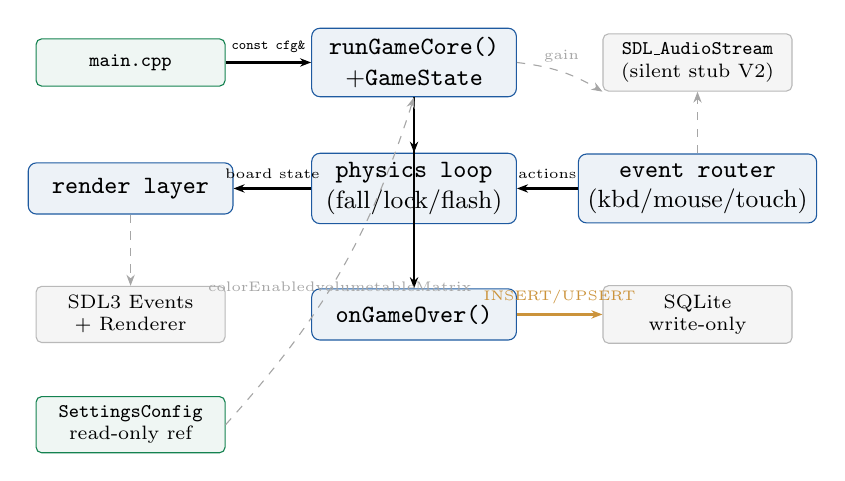
\begin{tikzpicture}[
  comp/.style={rectangle,draw=pillarBlue,fill=pillarBlue!8,rounded corners=3pt,
               minimum width=2.6cm,minimum height=0.65cm,align=center,font=\small},
  ext/.style={rectangle,draw=gray!55,fill=gray!8,rounded corners=2pt,
              minimum width=2.4cm,minimum height=0.6cm,align=center,font=\scriptsize},
  ro/.style={rectangle,draw=versionGreen,fill=versionGreen!7,rounded corners=2pt,
             minimum width=2.4cm,minimum height=0.6cm,align=center,font=\scriptsize},
  iface/.style={-{Stealth[length=4pt]},thick},
  use/.style={-{Stealth[length=4pt]},dashed,gray!70},
  write/.style={-{Stealth[length=4pt]},thick,versionAmber!80}
]
  \node[ro](main)  at (0,0)    {\texttt{main.cpp}};
  \node[comp](entry) at (3.6,0) {\texttt{runGameCore()}\\+\texttt{GameState}};
  \node[comp](phys) at (3.6,-1.6){\texttt{physics loop}\\(fall/lock/flash)};
  \node[comp](rend) at (0,-1.6) {\texttt{render layer}};
  \node[comp](inp)  at (7.2,-1.6){\texttt{event router}\\(kbd/mouse/touch)};
  \node[comp](ogo)  at (3.6,-3.2){\texttt{onGameOver()}};
  \node[ext](sdl)   at (0,-3.2) {SDL3 Events\\+ Renderer};
  \node[ext](bgm)   at (7.2,0)  {\texttt{SDL\_AudioStream}\\(silent stub V2)};
  \node[ext](dbw)   at (7.2,-3.2){SQLite\\write-only};
  \node[ro](cfg)    at (0,-4.6) {\texttt{SettingsConfig}\\read-only ref};

  \draw[iface](main)--node[above,font=\tiny]{\texttt{const cfg\&}}(entry);
  \draw[iface](entry)--(phys);
  \draw[iface](phys)--(rend) node[above,font=\tiny,midway]{board state};
  \draw[iface](inp)--(phys)  node[above,font=\tiny,midway]{actions};
  \draw[iface](entry)--(ogo);
  \draw[write](ogo.east)--node[above,font=\tiny]{INSERT/UPSERT}(dbw.west);
  \draw[use](rend)--(sdl);
  \draw[use](inp.north)--(bgm.south);
  \draw[use](entry.east)to[bend left=12]node[above,font=\tiny]{gain}(bgm.south west);
  \draw[use](cfg.east)to[bend right=12]
      node[below,font=\tiny]{colorEnabled\\volume\\tableMatrix}(entry.south);
\end{tikzpicture}
\end{center}

\noindent\textbf{State machine (flag-based transitions):}

\begin{center}
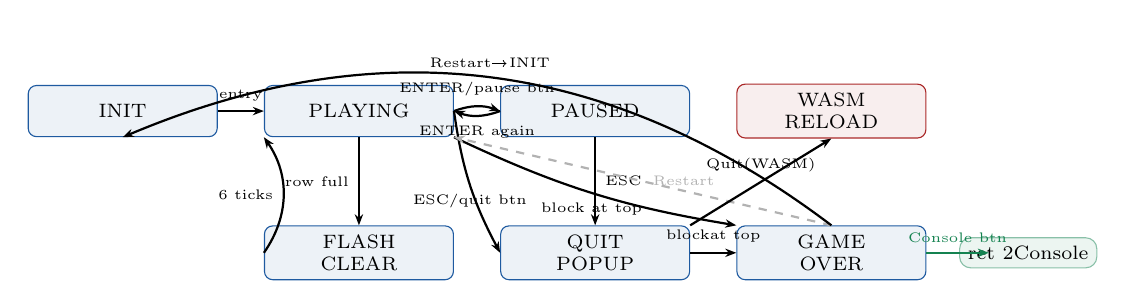
\begin{tikzpicture}[
  st/.style={rectangle,draw=pillarBlue,fill=pillarBlue!8,rounded corners=3pt,
             minimum width=2.4cm,minimum height=0.65cm,align=center,font=\scriptsize},
  wasm/.style={rectangle,draw=versionRed,fill=versionRed!8,rounded corners=3pt,
               minimum width=2.4cm,minimum height=0.65cm,align=center,font=\scriptsize},
  arr/.style={-{Stealth[length=4pt]},thick},
  darr/.style={-{Stealth[length=4pt]},dashed,gray!60,thick}
]
  \node[st](init)  at (0,0)       {INIT};
  \node[st](play)  at (3.0,0)     {PLAYING};
  \node[st](flash) at (3.0,-1.8)  {FLASH\\CLEAR};
  \node[st](pause) at (6.0,0)     {PAUSED};
  \node[st](popup) at (6.0,-1.8)  {QUIT\\POPUP};
  \node[st](over)  at (9.0,-1.8)  {GAME\\OVER};
  \node[wasm](wasm)at (9.0,0)     {WASM\\RELOAD};

  \draw[arr](init)--node[above,font=\tiny]{entry}(play);
  \draw[arr](play)--node[left,font=\tiny]{row full}(flash);
  \draw[arr](flash.west)to[bend right=35]
      node[left,font=\tiny]{6 ticks}(play.south west);
  \draw[arr](play.east)to[bend left=20]
      node[above,font=\tiny]{ENTER/pause btn}(pause.west);
  \draw[arr](pause.west)to[bend left=20]
      node[below,font=\tiny]{ENTER again}(play.east);
  \draw[arr](play.east)to[bend right=10]
      node[below,font=\tiny]{ESC/quit btn}(popup.west);
  \draw[arr](pause.south)--node[right,font=\tiny]{ESC}(popup.north);
  \draw[arr](popup.east)--node[above,font=\tiny]{block\\at top}(over.west);
  \draw[arr](play.south east)to[bend right=8]
      node[below,font=\tiny]{block at top}(over.north west);
  \draw[darr](over.north)--node[right,font=\tiny]{Restart}(play.south east);
  \draw[arr](over.north)to[bend right=30]
      node[above,font=\tiny]{Restart→INIT}(init.south);
  \draw[arr](popup.north east)--node[above,font=\tiny]{Quit\\(WASM)}(wasm.south);
  \node[font=\scriptsize,draw=versionGreen!50,fill=versionGreen!8,rounded corners,
        inner sep=3pt] at (11.5,-1.8) {ret 2\\Console};
  \draw[arr,versionGreen](over.east)--node[above,font=\tiny]{Console btn}(11.0,-1.8);
\end{tikzpicture}
\end{center}

% ─────────────────────────────────────────────────────────
\subsection{Thuật toán cốt lõi}

\subsubsection{spawnBlock() --- sinh khối ngẫu nhiên}

\begin{center}
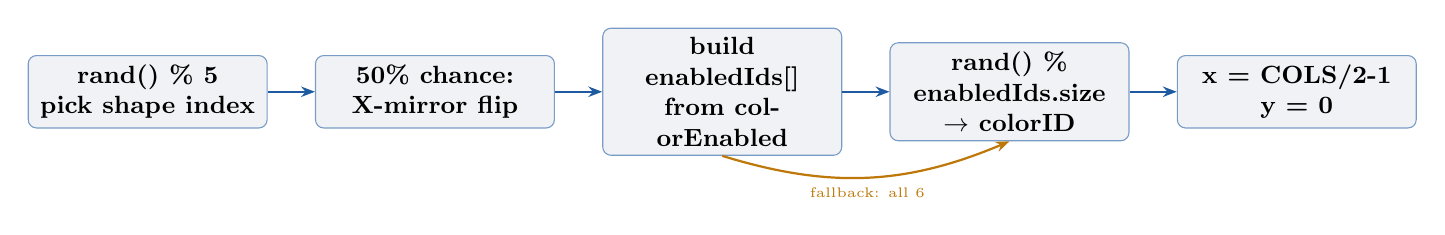
\begin{tikzpicture}[node distance=0.5cm,
  b/.style={sdsBox=pillarBlue!60,text width=2.8cm}]
  \node[b](a){rand() \% 5\\pick shape index};
  \node[b,right=0.6cm of a](b){50\% chance:\\X-mirror flip};
  \node[b,right=0.6cm of b](c){build\\enabledIds[]\\from colorEnabled};
  \node[b,right=0.6cm of c](d){rand() \%\\enabledIds.size\\$\rightarrow$ colorID};
  \node[b,right=0.6cm of d](e){x = COLS/2-1\\y = 0};
  \foreach \x/\y in {a/b,b/c,c/d,d/e}{\draw[sdsArrow=pillarBlue](\x)--(\y);}
  \draw[sdsArrow=versionAmber,bend right=20](c.south)to
      node[below,font=\tiny]{fallback: all 6}(d.south);
\end{tikzpicture}
\end{center}

\noindent\textbf{Mirror flip formula:} if \texttt{(rand() \& 1) == 0}:
$\texttt{blocks}[i].x = \texttt{maxX} - \texttt{blocks}[i].x$ for all 4 blocks.

\noindent\textbf{Color palette mapping} (\texttt{PALETTE\_TO\_COLOR[7]}):

\begin{center}\small
\begin{tabular}{@{}cll@{}}
\hline
\textbf{colorEnabled[i]} & \textbf{Màu} & \textbf{Ánh xạ \texttt{COLORS[]}} \\
\hline
0 & Đỏ (red)    & \texttt{COLORS[2]} \\
1 & Cam (orange)& \texttt{COLORS[5]} \\
2 & Hồng (pink) & \texttt{COLORS[7]} \\
3 & Vàng (yellow)&\texttt{COLORS[4]} \\
4 & Xanh lá (green)&\texttt{COLORS[3]} \\
5 & Xanh dương (blue)&\texttt{COLORS[1]} \\
6 & Tím (purple)& \texttt{COLORS[6]} \\
\hline
\end{tabular}
\end{center}

\subsubsection{checkCollision() \& rotated() --- vật lý khối}

\noindent\textbf{checkCollision} (matrix-based, O(4)):
\[
  \forall i \in [0,4):
  \quad nx = t.x + t.\texttt{blocks}[i].x,\;
        ny = t.y + t.\texttt{blocks}[i].y
\]
\[
  \text{collision} \iff nx < 0 \;\vee\; nx \geq \texttt{BOARD\_COLS}
    \;\vee\; ny \geq \texttt{BOARD\_ROWS}
    \;\vee\; (ny \geq 0 \wedge \texttt{board}[ny][nx] \neq 0)
\]

\noindent\textbf{rotated} (fixed pivot \texttt{(px,py)=(1,1)}):
\[
  \text{CW}: \begin{cases}
    x' = -\text{relY} + 1 \\
    y' = \phantom{-}\text{relX} + 1
  \end{cases}
  \qquad
  \text{CCW}: \begin{cases}
    x' = \phantom{-}\text{relY} + 1 \\
    y' = -\text{relX} + 1
  \end{cases}
  \quad \text{where relX/Y} = x/y - 1
\]

\subsubsection{Flash Clear Sequence --- lockBlock() $\rightarrow$ finishLineClear()}

\begin{center}
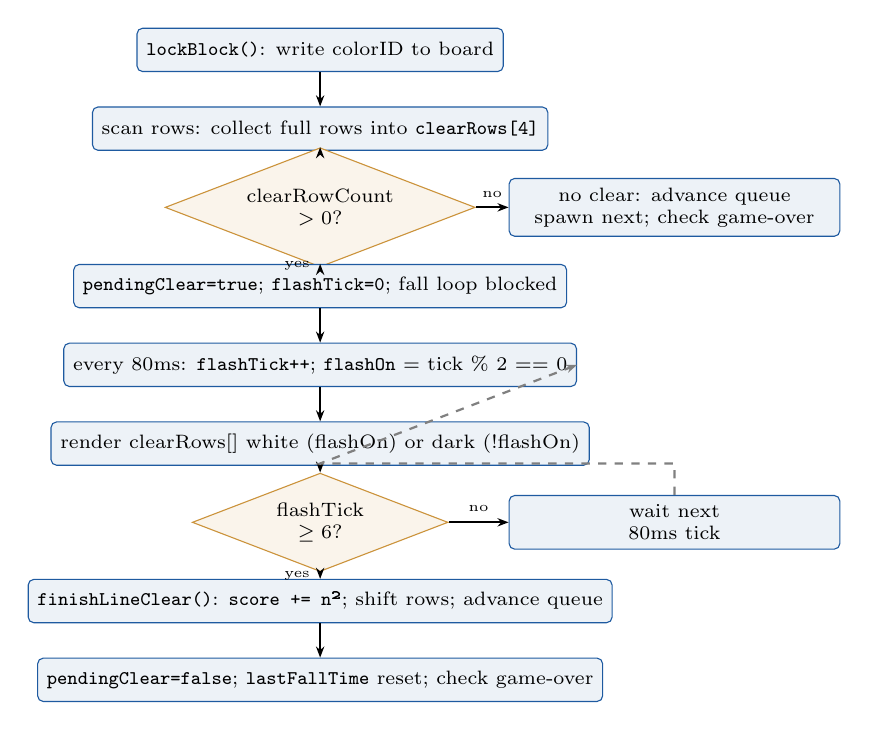
\begin{tikzpicture}[
  proc/.style={rectangle,draw=pillarBlue,fill=pillarBlue!8,rounded corners=2pt,
               minimum width=4.2cm,minimum height=0.55cm,align=center,font=\scriptsize},
  dec/.style={diamond,draw=versionAmber!80,fill=versionAmber!8,
              aspect=2.6,align=center,font=\scriptsize},
  arr/.style={-{Stealth[length=4pt]},thick}
]
  \node[proc](p0)  at (0,0)   {\texttt{lockBlock()}: write colorID to board};
  \node[proc](p1)  at (0,-1.0){scan rows: collect full rows into
                                \texttt{clearRows[4]}};
  \node[dec] (d0)  at (0,-2.0){clearRowCount\\$> 0$?};
  \node[proc](pnc) at (4.5,-2.0){no clear: advance queue\\spawn next; check game-over};
  \node[proc](p2)  at (0,-3.0){\texttt{pendingClear=true}; \texttt{flashTick=0};
                                fall loop blocked};
  \node[proc](p3)  at (0,-4.0){every 80ms: \texttt{flashTick++};
                                \texttt{flashOn} = tick \% 2 == 0};
  \node[proc](p4)  at (0,-5.0){render clearRows[]
                                white (flashOn) or dark (!flashOn)};
  \node[dec] (d1)  at (0,-6.0){flashTick\\$\geq 6$?};
  \node[proc](p5)  at (4.5,-6.0){wait next\\80ms tick};
  \node[proc](p6)  at (0,-7.0){\texttt{finishLineClear()}:
                                \texttt{score += n²}; shift rows; advance queue};
  \node[proc](p7)  at (0,-8.0){\texttt{pendingClear=false};
                                \texttt{lastFallTime} reset; check game-over};

  \draw[arr](p0)--(p1);\draw[arr](p1)--(d0);
  \draw[arr](d0)--node[above,font=\tiny]{no}(pnc);
  \draw[arr](d0)--node[left,font=\tiny]{yes}(p2);
  \draw[arr](p2)--(p3);\draw[arr](p3)--(p4);\draw[arr](p4)--(d1);
  \draw[arr](d1)--node[above,font=\tiny]{no}(p5);
  \draw[arr,gray,dashed](p5.north)--++(0,0.4)--++(-4.5,0)--(p3.east);
  \draw[arr](d1)--node[left,font=\tiny]{yes}(p6);\draw[arr](p6)--(p7);
\end{tikzpicture}
\end{center}

\noindent\textbf{Flash timing diagram} (6 ticks $\times$ 80\,ms $\approx$ 480\,ms):

\begin{center}
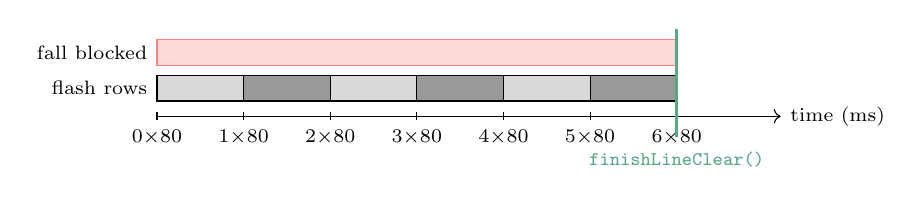
\begin{tikzpicture}[every node/.style={font=\scriptsize},x=1.1cm,y=0.65cm]
  \draw[->](0,0)--(7.2,0) node[right]{time (ms)};
  \foreach \x in {0,...,6}{
    \draw(\x,0.08)--(\x,-0.08) node[below]{\x$\times$80};
  }
  \foreach \x/\c in {0/white!70!gray,1/gray!80,2/white!70!gray,
                      3/gray!80,4/white!70!gray,5/gray!80}{
    \fill[\c](\x,0.3) rectangle (\x+1,0.8);
    \draw[black](\x,0.3) rectangle (\x+1,0.8);
  }
  \node[left] at (0,0.55){flash rows};
  \fill[red!15](0,1.0) rectangle (6,1.5);
  \draw[red!50](0,1.0) rectangle (6,1.5);
  \node[left] at (0,1.25){fall blocked};
  \draw[versionGreen!70,very thick](6,-0.4)--(6,1.7);
  \node[versionGreen!70,below] at (6,-0.5){\texttt{finishLineClear()}};
\end{tikzpicture}
\end{center}

\subsubsection{getFallInterval() --- dynamic speed}

\begin{center}
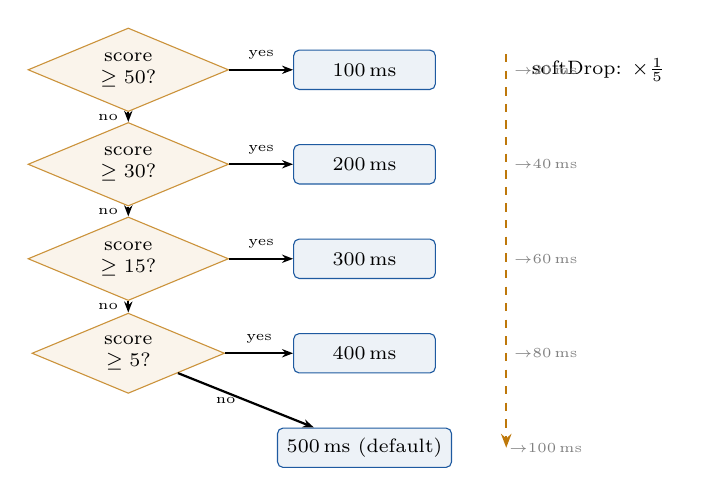
\begin{tikzpicture}[
  dec/.style={diamond,draw=versionAmber!80,fill=versionAmber!8,
              aspect=2.4,align=center,font=\scriptsize},
  val/.style={rectangle,draw=pillarBlue,fill=pillarBlue!8,rounded corners=2pt,
              minimum width=1.8cm,minimum height=0.5cm,align=center,font=\scriptsize},
  arr/.style={-{Stealth[length=4pt]},thick}
]
  \node[dec](d0) at (0,0)    {score\\$\geq 50$?};
  \node[dec](d1) at (0,-1.2) {score\\$\geq 30$?};
  \node[dec](d2) at (0,-2.4) {score\\$\geq 15$?};
  \node[dec](d3) at (0,-3.6) {score\\$\geq 5$?};
  \node[val](v100) at (3.0,0)   {100\,ms};
  \node[val](v200) at (3.0,-1.2){200\,ms};
  \node[val](v300) at (3.0,-2.4){300\,ms};
  \node[val](v400) at (3.0,-3.6){400\,ms};
  \node[val](v500) at (3.0,-4.8){500\,ms (default)};
  \foreach \d/\v in {d0/v100,d1/v200,d2/v300,d3/v400}{
    \draw[arr](\d)--node[above,font=\tiny]{yes}(\v);
  }
  \foreach \d/\dn in {d0/d1,d1/d2,d2/d3}{
    \draw[arr](\d)--node[left,font=\tiny]{no}(\dn);
  }
  \draw[arr](d3)--node[left,font=\tiny]{no}(v500);
  \node[font=\scriptsize,right=0.2cm of v100] at (4.8,0)
      {softDrop: $\times\frac{1}{5}$};
  \draw[sdsArrow=versionAmber,dashed](4.8,0.2)--(4.8,-4.8);
  \foreach \y/\v in {0/20, -1.2/40, -2.4/60, -3.6/80, -4.8/100}{
    \node[font=\tiny,gray] at (5.3,\y){$\rightarrow$\v\,ms};
  }
\end{tikzpicture}
\end{center}

\subsubsection{Elapsed Time Calculation (Pause-aware)}

\noindent Computed every frame from \texttt{GameState} fields:
\[
  \texttt{elapsedMs} = \begin{cases}
    \texttt{nowMs} - \texttt{gameStartTime} - \texttt{totalPausedMs}
      & \text{if } \texttt{nowRunning} \\[4pt]
    \texttt{pauseStartTime} - \texttt{gameStartTime} - \texttt{totalPausedMs}
      & \text{otherwise (frozen display)}
  \end{cases}
\]

\noindent\textbf{Pause transition bookkeeping:}
\begin{enumerate}[nosep,label=\arabic*.]
  \item \texttt{wasRunning = true} $\rightarrow$ \texttt{nowRunning = false}:
        capture \texttt{pauseStartTime = nowMs}.
  \item \texttt{wasRunning = false} $\rightarrow$ \texttt{nowRunning = true}:
        \texttt{totalPausedMs += nowMs - pauseStartTime}.
  \item \texttt{wasRunning = nowRunning} (no change): no-op.
\end{enumerate}

\subsubsection{applyTableMatrix() --- board pre-population}

\noindent Format: \texttt{";"-separated rows (bottom-aligned), ","-separated
colorID values (0=empty, 1--7=colors)}.

\begin{center}
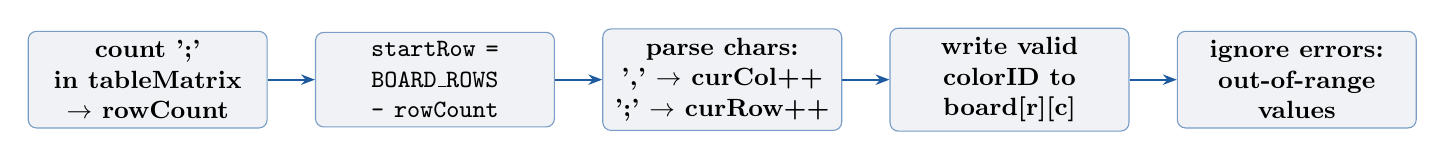
\begin{tikzpicture}[node distance=0.5cm,
  b/.style={sdsBox=pillarBlue!60,text width=2.8cm}]
  \node[b](a){count ';'\\in tableMatrix\\$\rightarrow$ rowCount};
  \node[b,right=0.6cm of a](b){\texttt{startRow =}\\
                                 \texttt{BOARD\_ROWS}\\
                                 \texttt{- rowCount}};
  \node[b,right=0.6cm of b](c){parse chars:\\',' $\rightarrow$ curCol++\\';' $\rightarrow$ curRow++};
  \node[b,right=0.6cm of c](d){write valid\\colorID to\\board[r][c]};
  \node[b,right=0.6cm of d](e){ignore errors:\\out-of-range\\values};
  \foreach \x/\y in {a/b,b/c,c/d,d/e}{\draw[sdsArrow=pillarBlue](\x)--(\y);}
\end{tikzpicture}
\end{center}

\noindent\textbf{Empty string} (\texttt{""}) $\rightarrow$ blank board; parse error per cell $\rightarrow$ silently skip (no crash). Called in \texttt{resetGame()} \textbf{after} \texttt{srand} and \textbf{before} first \texttt{spawnBlock()}.

\subsubsection{Swipe Gesture Recognition}

\begin{center}
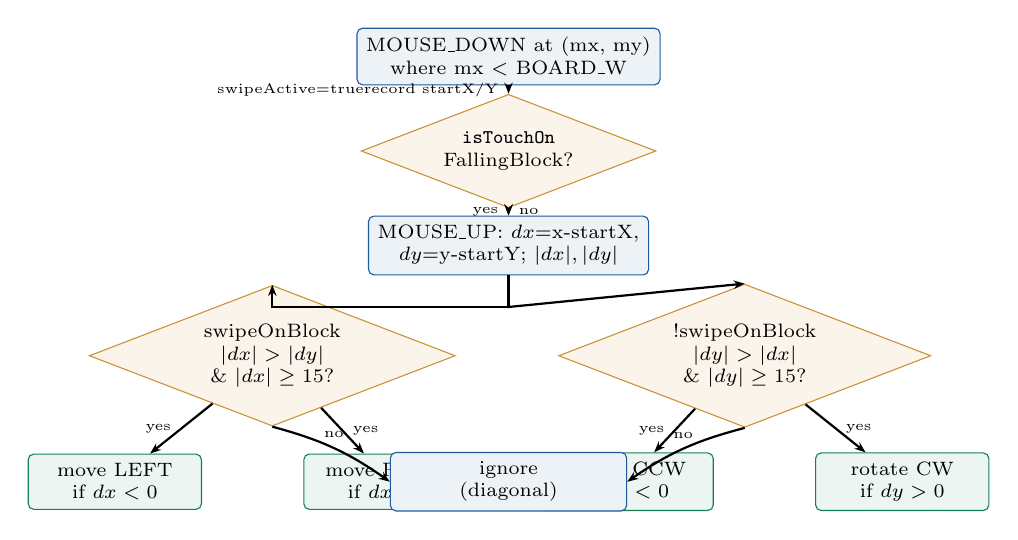
\begin{tikzpicture}[
  dec/.style={diamond,draw=versionAmber!80,fill=versionAmber!8,
              aspect=2.6,align=center,font=\scriptsize},
  act/.style={rectangle,draw=versionGreen,fill=versionGreen!8,rounded corners=2pt,
              minimum width=2.2cm,minimum height=0.5cm,align=center,font=\scriptsize},
  proc/.style={rectangle,draw=pillarBlue,fill=pillarBlue!8,rounded corners=2pt,
               minimum width=3.0cm,minimum height=0.5cm,align=center,font=\scriptsize},
  arr/.style={-{Stealth[length=4pt]},thick}
]
  \node[proc](p0) at (0,0)    {MOUSE\_DOWN at (mx, my)\\where mx $<$ BOARD\_W};
  \node[dec] (d0) at (0,-1.2) {\texttt{isTouchOn}\\FallingBlock?};
  \node[proc](p1) at (0,-2.4) {MOUSE\_UP: $dx$=x-startX,\\$dy$=y-startY;
                                 $|dx|,|dy|$};
  \node[dec] (d1) at (-3.0,-3.8){swipeOnBlock\\$|dx|>|dy|$\\$\&$ $|dx|\geq 15$?};
  \node[dec] (d2) at (3.0,-3.8){!swipeOnBlock\\$|dy|>|dx|$\\$\&$ $|dy|\geq 15$?};
  \node[act](left)  at (-5.0,-5.4){move LEFT\\if $dx<0$};
  \node[act](right) at (-1.5,-5.4){move RIGHT\\if $dx>0$};
  \node[act](up)    at (1.5,-5.4) {rotate CCW\\if $dy<0$};
  \node[act](down)  at (5.0,-5.4) {rotate CW\\if $dy>0$};
  \node[proc](ign)  at (0,-5.4)   {ignore\\(diagonal)};

  \draw[arr](p0)--node[left,font=\tiny]{swipeActive=true\\record startX/Y}(d0);
  \draw[arr](d0)--node[left,font=\tiny]{yes}(p1);
  \draw[arr](d0)--node[right,font=\tiny]{no}(p1);
  \draw[arr](p1.south)--++(0,-0.4)--++(-3.0,0)--(d1.north);
  \draw[arr](p1.south)--++(0,-0.4)--(d2.north);
  \draw[arr](d1)--node[left,font=\tiny]{yes}(left);
  \draw[arr](d1)--node[right,font=\tiny]{yes}(right);
  \draw[arr](d2)--node[left,font=\tiny]{yes}(up);
  \draw[arr](d2)--node[right,font=\tiny]{yes}(down);
  \draw[arr](d1.south)to[bend left=10]node[above,font=\tiny]{no}(ign.west);
  \draw[arr](d2.south)to[bend right=10]node[above,font=\tiny]{no}(ign.east);
\end{tikzpicture}
\end{center}

% ─────────────────────────────────────────────────────────
\subsection{Cấu trúc dữ liệu}

\subsubsection{C++ Structs}

\begin{verbatim}
// gameCore_layout.h
struct Point     { int x, y; };
struct Tetromino { Point blocks[4]; int colorID; int x, y; };

struct GameState {
    int       board[BOARD_ROWS][BOARD_COLS] = {0};  // 0=empty, 1-7=colorID
    Tetromino currentBlock, nextBlock, nextBlock2, nextBlock3;
    int  score=0, exitCode=0, retryCount=0;
    bool isGameOver=false, isPaused=false, showQuitPopup=false;
    bool softDrop=false, speedHeld=false;
    // flash-clear
    bool pendingClear=false; int clearRowCount=0;
    int  clearRows[4]; int flashTick=0; bool flashOn=false;
    Uint32 flashTimer=0;
    // pause-aware timer
    Uint32 gameStartTime=0, pauseStartTime=0, totalPausedMs=0;
    bool   wasRunning=false;
    // sidebar mouse hold flags (highlight yellow effect)
    bool mouseHeldQuit, mouseHeldPause, mouseHeld{ArrUp,Down,Left,Right};
    // WASM
    bool wasmShutdown=false, reloadHover=false;
};
\end{verbatim}

\subsubsection{Layout Constants \& Sidebar Map}

\begin{center}\small
\begin{tabular}{@{}l r r l@{}}
\hline
\textbf{Constant} & \textbf{Value} & \textbf{Formula} & \textbf{Meaning} \\
\hline
\texttt{BOARD\_COLS}  & 10 & --  & grid columns \\
\texttt{BOARD\_ROWS}  & 20 & --  & grid rows \\
\texttt{BLOCK\_SIZE}  & 24 & --  & px per cell \\
\texttt{BLOCK\_PAD}   &  1 & --  & inner padding \\
\texttt{BOARD\_W}     & 240 & 10×24 & board pixel width \\
\texttt{SIDEBAR\_X}   & 240 & BOARD\_W & sidebar left edge \\
\texttt{SIDEBAR\_W}   &  30 & 270-240 & sidebar width \\
\texttt{COMP\_H}      &  40 & -- & slot height (12×40=480) \\
\hline
\end{tabular}
\end{center}

\noindent\textbf{Sidebar slot map} (\texttt{rectAt(i) = \{240, i*40, 30, 40\}}):

\begin{center}\small
\begin{tabular}{@{}c l l@{}}
\hline
\textbf{Slot} & \textbf{Name} & \textbf{Content / Icon} \\
\hline
0 & QUIT      & Power-off icon (circular arc + vertical bar) \\
1 & PAUSE     & Square (playing) $\leftrightarrow$ triangle (paused) \\
2 & SCORE     & \texttt{"\%05d"} at 0.65 scale (5 chars $\times$ 8px $\times$ 0.65) \\
3 & TIMER     & \texttt{"\%02d:\%02d"} (HH:MM) at 0.65 scale \\
4 & NEXT-1    & Always visible; + story label \texttt{"S\{id\}-C\{id\}"} overlay \\
5 & NEXT-2    & Visible if \texttt{nextBlockScore>0 \&\& score$\geq$nextBlockScore} \\
6 & NEXT-3    & Visible if NEXT-2 open \&\& \texttt{score$\geq$nextBlockScore$\times$2} \\
7 & ARR UP    & CCW rotate arrow \\
8 & ARR DOWN  & CW rotate arrow \\
9 & ARR LEFT  & Move left arrow \\
10 & ARR RIGHT & Move right arrow \\
11 & SPEED    & Double chevron $\gg$ booster icon \\
\hline
\end{tabular}
\end{center}

\subsubsection{DB Write Boundary Diagram}

\noindent gameCore does \textbf{not own} any DB table; it only writes to tables
created and owned by gameConsole.

\begin{center}
% Lesson: define \pk locally inside center block
\newcommand{\pk}[1]{\underline{#1}}
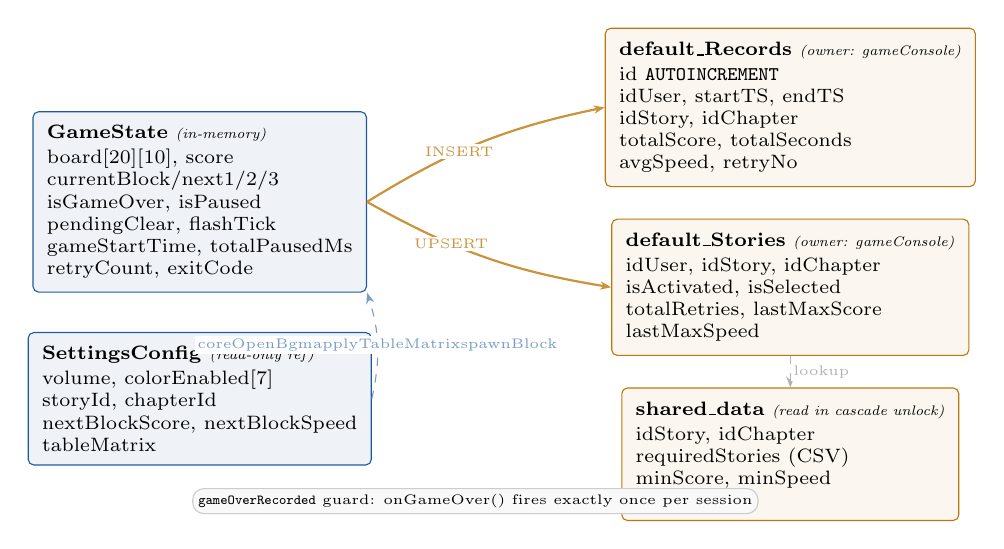
\begin{tikzpicture}[
  inmem/.style={rectangle,draw=pillarBlue,fill=pillarBlue!7,rounded corners=2pt,
                align=left,font=\scriptsize,inner sep=5pt,minimum width=3.4cm},
  owned/.style={rectangle,draw=versionAmber,fill=versionAmber!6,rounded corners=2pt,
                align=left,font=\scriptsize,inner sep=5pt,minimum width=3.4cm},
  write/.style={-{Stealth[length=4pt]},thick,versionAmber!80},
  read/.style={-{Stealth[length=4pt]},dashed,gray!60},
  lbl/.style={font=\tiny,fill=white,inner sep=1pt}
]
  % in-memory (left)
  \node[inmem](gs) at (0,0) {
    \textbf{GameState}\ \textit{\tiny(in-memory)}\\[1pt]
    board[20][10], score\\
    currentBlock/next1/2/3\\
    isGameOver, isPaused\\
    pendingClear, flashTick\\
    gameStartTime, totalPausedMs\\
    retryCount, exitCode
  };
  \node[inmem,below=0.5cm of gs](cfg) {
    \textbf{SettingsConfig}\ \textit{\tiny(read-only ref)}\\[1pt]
    volume, colorEnabled[7]\\
    storyId, chapterId\\
    nextBlockScore, nextBlockSpeed\\
    tableMatrix
  };

  % DB write targets (right, owned by gameConsole)
  \node[owned](rec) at (7.5,1.2) {
    \textbf{default\_Records}\ \textit{\tiny(owner: gameConsole)}\\[1pt]
    \pk{id}\ \texttt{AUTOINCREMENT}\\
    idUser, startTS, endTS\\
    idStory, idChapter\\
    totalScore, totalSeconds\\
    avgSpeed, retryNo
  };
  \node[owned,below=0.4cm of rec](stor) {
    \textbf{default\_Stories}\ \textit{\tiny(owner: gameConsole)}\\[1pt]
    \pk{idUser, idStory, idChapter}\\
    isActivated, isSelected\\
    totalRetries, lastMaxScore\\
    lastMaxSpeed
  };
  \node[owned,below=0.4cm of stor](sd) {
    \textbf{shared\_data}\ \textit{\tiny(read in cascade unlock)}\\[1pt]
    \pk{idStory, idChapter}\\
    requiredStories (CSV)\\
    minScore, minSpeed\\
    minRetries
  };

  % write arrows (via onGameOver)
  \draw[write](gs.east)to[bend left=10]
      node[lbl,pos=0.4]{INSERT}(rec.west);
  \draw[write](gs.east)to[bend right=10]
      node[lbl,pos=0.35]{UPSERT}(stor.west);

  % cfg feeds gs
  \draw[read,pillarBlue!60](cfg.east)to[bend right=15]
      node[lbl,pos=0.5]{coreOpenBgm\\applyTableMatrix\\spawnBlock}(gs.south east);

  % cascade unlock
  \draw[read](stor.south)--node[lbl,right]{lookup}(sd.north);

  % guard note
  \node[font=\tiny,draw=gray!40,fill=gray!5,rounded corners,inner sep=2pt]
    at (3.5,-3.8)
    {\texttt{gameOverRecorded} guard: onGameOver() fires exactly once per session};
\end{tikzpicture}
\end{center}

\subsubsection{Dataflow Diagram --- Game Loop}

\begin{center}
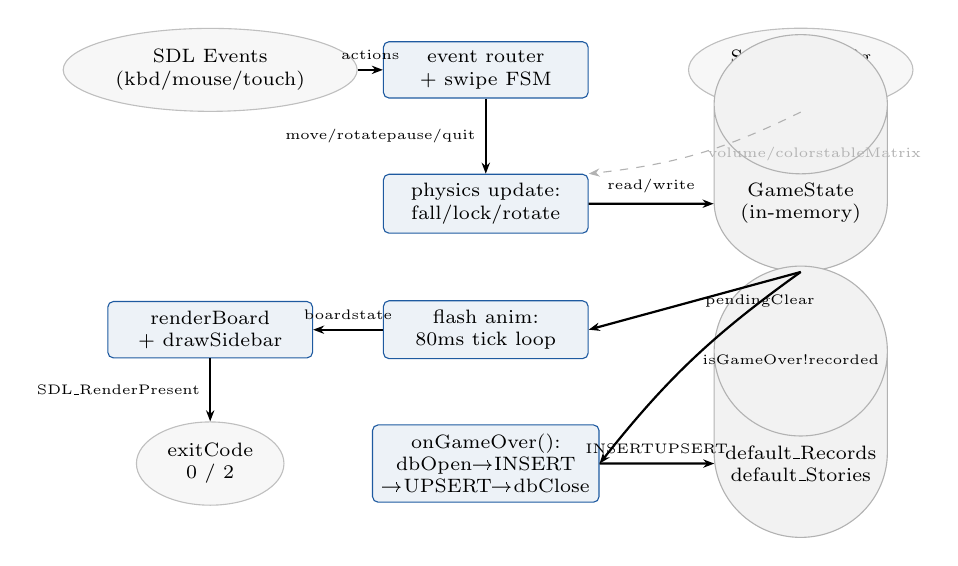
\begin{tikzpicture}[
  proc/.style={rectangle,draw=pillarBlue,fill=pillarBlue!8,rounded corners=2pt,
               minimum width=2.6cm,minimum height=0.6cm,align=center,font=\scriptsize},
  store/.style={cylinder,draw=gray!60,fill=gray!10,shape border rotate=90,
                minimum width=2.2cm,minimum height=0.55cm,align=center,font=\scriptsize},
  extio/.style={ellipse,draw=gray!50,fill=gray!6,minimum width=1.8cm,
                minimum height=0.5cm,align=center,font=\scriptsize},
  fl/.style={-{Stealth[length=4pt]},thick},
  dfl/.style={-{Stealth[length=4pt]},dashed,gray!60}
]
  \node[extio](ev)   at (0,5.5)  {SDL Events\\(kbd/mouse/touch)};
  \node[extio](cfg2) at (7.5,5.5){SettingsConfig\\(read-only)};
  \node[proc](route) at (3.5,5.5){event router\\+ swipe FSM};
  \node[proc](phys2) at (3.5,3.8){physics update:\\fall/lock/rotate};
  \node[store](gs2)  at (7.5,3.8){GameState\\(in-memory)};
  \node[proc](flash2)at (3.5,2.2){flash anim:\\80ms tick loop};
  \node[proc](rend3) at (0,2.2)  {renderBoard\\+ drawSidebar};
  \node[proc](ogo)   at (3.5,0.5){onGameOver():\\dbOpen→INSERT\\→UPSERT→dbClose};
  \node[store](db3)  at (7.5,0.5){default\_Records\\default\_Stories};
  \node[extio](ret2) at (0,0.5)  {exitCode\\0 / 2};

  \draw[fl](ev)--node[above,font=\tiny]{actions}(route);
  \draw[fl](route)--node[left,font=\tiny]{move/rotate\\pause/quit}(phys2);
  \draw[fl](phys2)--node[above,font=\tiny]{read/write}(gs2);
  \draw[fl](gs2.south)--node[right,font=\tiny]{pendingClear}(flash2.east);
  \draw[fl](flash2)--node[above,font=\tiny]{board\\state}(rend3);
  \draw[fl](gs2.south)to[bend right=8]
      node[right,font=\tiny]{isGameOver\\!recorded}(ogo.east);
  \draw[fl](ogo.east)--node[above,font=\tiny]{INSERT\\UPSERT}(db3.west);
  \draw[fl](rend3.south)--node[left,font=\tiny]{SDL\_Render\\Present}(ret2.north);
  \draw[dfl](cfg2.south)to[bend left=10]
      node[right,font=\tiny]{volume/colors\\tableMatrix}(phys2.north east);
\end{tikzpicture}
\end{center}

\subsubsection{Sequence Diagram --- Entry, Flash-clear, Game-over DB}

\begin{center}
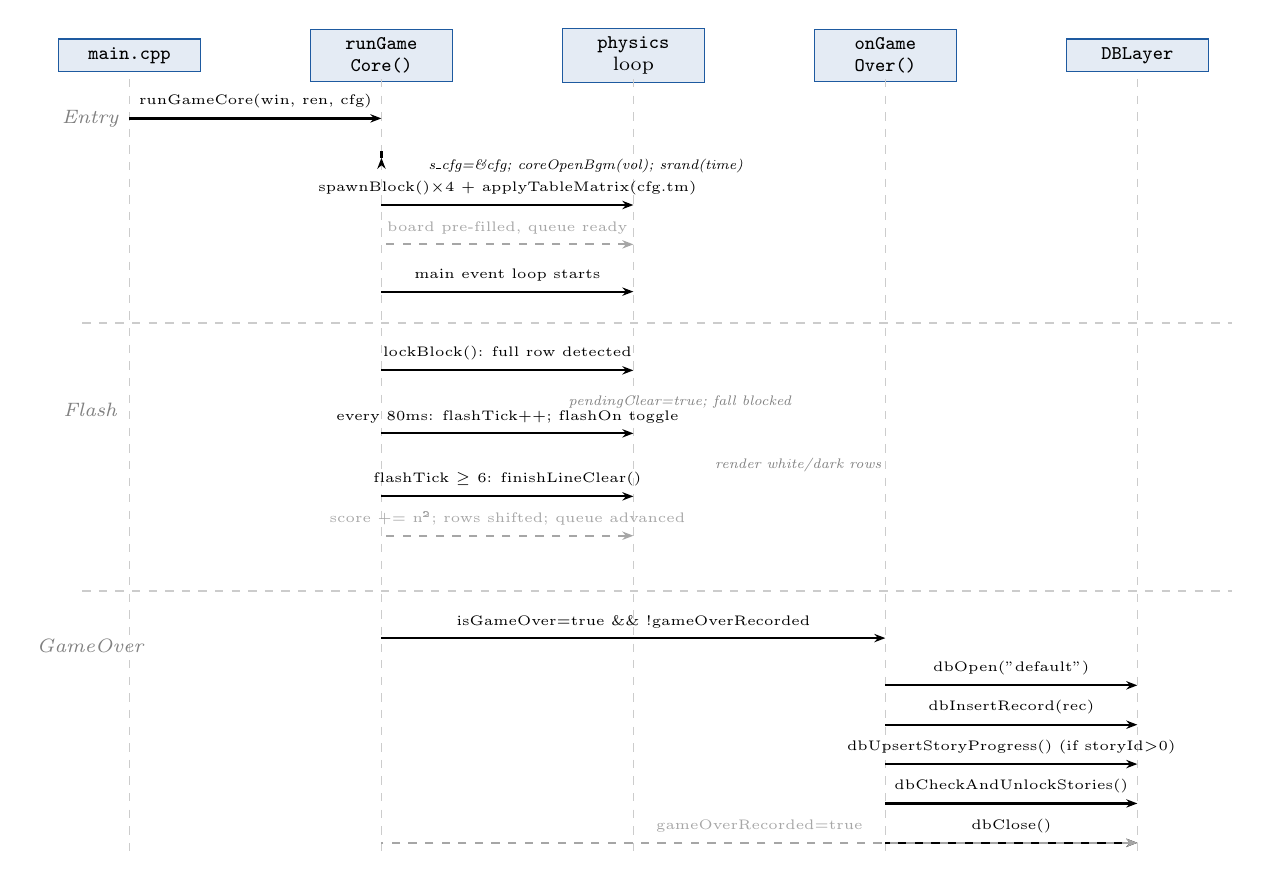
\begin{tikzpicture}[
  lhd/.style={rectangle,fill=pillarBlue!12,draw=pillarBlue,font=\scriptsize,
              inner sep=3pt,minimum width=1.8cm,align=center},
  msg/.style={-{Stealth[length=4pt]},thick},
  ret/.style={{Stealth[length=4pt]}-,thick,dashed,gray!70},
  lf/.style={draw=gray!40,dashed}
]
  \node[lhd](H1) at (0,0)    {\texttt{main.cpp}};
  \node[lhd](H2) at (3.2,0)  {\texttt{runGame}\\\texttt{Core()}};
  \node[lhd](H3) at (6.4,0)  {\texttt{physics}\\loop};
  \node[lhd](H4) at (9.6,0)  {\texttt{onGame}\\\texttt{Over()}};
  \node[lhd](H5) at (12.8,0) {\texttt{DBLayer}};

  \foreach \x in {0,3.2,6.4,9.6,12.8}{\draw[lf](\x,-0.3)--(\x,-10.2);}

  % dividers
  \draw[gray!40,thick,dashed](-0.6,-3.4)--(14,-3.4);
  \draw[gray!40,thick,dashed](-0.6,-6.8)--(14,-6.8);
  \node[font=\scriptsize\itshape,gray] at (-0.5,-0.8){Entry};
  \node[font=\scriptsize\itshape,gray] at (-0.5,-4.5){Flash};
  \node[font=\scriptsize\itshape,gray] at (-0.5,-7.5){GameOver};

  % ── Entry ──
  \draw[msg](0,-0.8)--(3.2,-0.8)
      node[above,font=\tiny,midway]{runGameCore(win, ren, cfg)};
  \draw[msg](3.2,-1.3)--(3.2,-1.3);
  \node[font=\tiny,align=center] at (5.8,-1.4)
      {\textit{s\_cfg=\&cfg; coreOpenBgm(vol); srand(time)}};
  \draw[msg](3.2,-1.9)--(6.4,-1.9)
      node[above,font=\tiny,midway]{spawnBlock()$\times$4 + applyTableMatrix(cfg.tm)};
  \draw[ret](6.4,-2.4)--(3.2,-2.4)
      node[above,font=\tiny,midway]{board pre-filled, queue ready};
  \draw[msg](3.2,-3.0)--(6.4,-3.0)
      node[above,font=\tiny,midway]{main event loop starts};

  % ── Flash-clear ──
  \draw[msg](3.2,-4.0)--(6.4,-4.0)
      node[above,font=\tiny,midway]{lockBlock(): full row detected};
  \node[font=\tiny,gray] at (7.0,-4.4){\textit{pendingClear=true; fall blocked}};
  \draw[msg](3.2,-4.8)--(6.4,-4.8)
      node[above,font=\tiny,midway]{every 80ms: flashTick++; flashOn toggle};
  \node[font=\tiny,gray] at (8.5,-5.2){\textit{render white/dark rows}};
  \draw[msg](3.2,-5.6)--(6.4,-5.6)
      node[above,font=\tiny,midway]{flashTick $\geq$ 6: finishLineClear()};
  \draw[ret](6.4,-6.1)--(3.2,-6.1)
      node[above,font=\tiny,midway]{score += n²; rows shifted; queue advanced};

  % ── Game-over DB ──
  \draw[msg](3.2,-7.4)--(9.6,-7.4)
      node[above,font=\tiny,midway]{isGameOver=true \&\& !gameOverRecorded};
  \draw[msg](9.6,-8.0)--(12.8,-8.0)
      node[above,font=\tiny,midway]{dbOpen("default")};
  \draw[msg](9.6,-8.5)--(12.8,-8.5)
      node[above,font=\tiny,midway]{dbInsertRecord(rec)};
  \draw[msg](9.6,-9.0)--(12.8,-9.0)
      node[above,font=\tiny,midway]{dbUpsertStoryProgress() (if storyId$>$0)};
  \draw[msg](9.6,-9.5)--(12.8,-9.5)
      node[above,font=\tiny,midway]{dbCheckAndUnlockStories()};
  \draw[msg](9.6,-10.0)--(12.8,-10.0)
      node[above,font=\tiny,midway]{dbClose()};
  \draw[ret](12.8,-10.0)--(3.2,-10.0)
      node[above,font=\tiny,midway]{gameOverRecorded=true};
\end{tikzpicture}
\end{center}

% ─────────────────────────────────────────────────────────
\subsection{Giao diện công khai}

\begin{verbatim}
// extern declared in app/main.cpp
int runGameCore(SDL_Window*          window,
                SDL_Renderer*        renderer,
                const SettingsConfig& cfg);
// Returns: 0 = quit/window-close | 2 = back to Console
// cfg: READ-ONLY — gameCore never modifies SettingsConfig.
// DB: opens and closes connection inside onGameOver() only.
//     Does NOT keep a DB handle across frames.
\end{verbatim}

\noindent\textbf{DB contract:} gameCore calls \texttt{dbOpen}/\texttt{dbClose}
per game-over event. Console's \texttt{g\_db} handle is a separate
\texttt{sqlite3*} — no double-open conflict.
\texttt{gameOverRecorded} (local \texttt{bool}) ensures exactly one
\texttt{onGameOver()} per session regardless of which exit path fires
(game-over auto, Restart, Console, Quit).

% ─────────────────────────────────────────────────────────
\subsection{Thư viện phụ thuộc}

\begin{tabularx}{\linewidth}{@{}l l X@{}}
\hline
\textbf{Thư viện} & \textbf{Guard} & \textbf{Vai trò} \\
\hline
SDL3              & always & Window, renderer, events, \texttt{SDL\_AudioStream},
                             \texttt{SDL\_GetKeyboardState} \\
sqlite3           & always & Write-only via \texttt{gameConsole\_db.h} (no direct
                             \texttt{sqlite3\_*} calls in app.cpp) \\
\texttt{gameConsole\_db.h} & always & DB API contract: \texttt{dbOpen/Close},
                              \texttt{dbInsertRecord}, \texttt{dbUpsertStoryProgress},
                              \texttt{dbCheckAndUnlockStories} \\
\texttt{gameConsole\_layout.h} & always & \texttt{SettingsConfig} definition \\
Emscripten        & \texttt{\#ifdef \_\_EMSCRIPTEN\_\_} &
  \texttt{emscripten\_run\_script("window.location.reload()")} for WASM reload \\
\hline
\end{tabularx}

\noindent\textbf{Zero-dependency goal (core logic):} collision detection,
rotation, line-clear, scoring, timer — all pure C++ with \texttt{<cstdlib>},
\texttt{<ctime>}, \texttt{<cmath>}. SDL3 and DB only in render/IO/persist layers.

\PartVersions

\begin{VersionTable}
\Vone & 5 shapes + mirror flip; keyboard/mouse/swipe; pause; WASM reload
      & SDL3
      & Reads \texttt{SettingsConfig\&} (defaults); no DB \\
\Vtwo & Dynamic speed; n² combo; flash-clear; 3-block queue;
        color palette; tableMatrix; DB write on game-over; BGM stub
      & sqlite3 (via gameConsole\_db.h)
      & Writes \texttt{default\_Records}; triggers cascade unlock \\
\Vthree & D1 leaderboard push; BGM real audio; name input; nextBlockScore3
        & libcurl / emscripten\_fetch
        & POST to Cloudflare Worker after each game-over \\
\end{VersionTable}

% ─────────────────────────────────────────────────────────
\subsection{\Vone\ --- Core Physics Engine}

\textbf{Mục tiêu:} Tetromino physics, 3-channel input, pause, popup, WASM reload.

\noindent\textbf{Screen layout pixel-map (270×480):}

\begin{center}
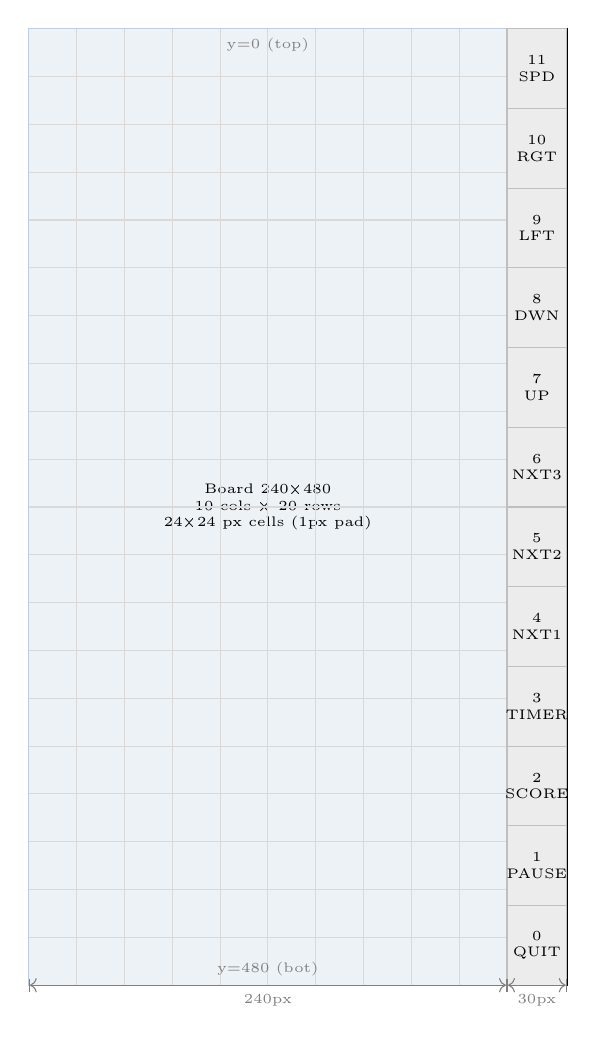
\begin{tikzpicture}[x=0.72pt,y=0.72pt,every node/.style={font=\tiny}]
  \draw[thick](0,0) rectangle (270,480);
  % board area
  \fill[pillarBlue!8](0,0) rectangle (240,480);
  \draw[pillarBlue!30](0,0) rectangle (240,480);
  \node[align=center] at (120,240){Board 240×480\\10 cols × 20 rows\\24×24 px cells (1px pad)};
  % grid lines hint
  \foreach \x in {24,48,72,96,120,144,168,192,216}{
    \draw[gray!30](\x,0)--(\x,480);
  }
  \foreach \y in {24,48,72,96,120,144,168,192,216,240,264,288,312,336,360,384,408,432,456}{
    \draw[gray!30](0,\y)--(240,\y);
  }
  % sidebar slots
  \foreach \s in {0,...,11}{
    \fill[gray!15](240,\s*40) rectangle (270,\s*40+40);
    \draw[gray!50](240,\s*40) rectangle (270,\s*40+40);
  }
  \node[align=center] at (255,20){0\\QUIT};
  \node[align=center] at (255,60){1\\PAUSE};
  \node[align=center] at (255,100){2\\SCORE};
  \node[align=center] at (255,140){3\\TIMER};
  \node[align=center] at (255,180){4\\NXT1};
  \node[align=center] at (255,220){5\\NXT2};
  \node[align=center] at (255,260){6\\NXT3};
  \node[align=center] at (255,300){7\\UP};
  \node[align=center] at (255,340){8\\DWN};
  \node[align=center] at (255,380){9\\LFT};
  \node[align=center] at (255,420){10\\RGT};
  \node[align=center] at (255,460){11\\SPD};
  % dimension labels
  \node[gray] at (120,472){y=0 (top)};
  \node[gray] at (120,8){y=480 (bot)};
  \draw[|<->|,gray](0,0)--(240,0) node[midway,below,font=\tiny]{240px};
  \draw[|<->|,gray](240,0)--(270,0) node[midway,below,font=\tiny]{30px};
\end{tikzpicture}
\end{center}

\noindent\textbf{I/O validation:}
\begin{itemize}[nosep]
  \item \texttt{spawnBlock()} with all \texttt{colorEnabled[i]=true}:
        color drawn from 7 options; never \texttt{colorID=0}.
  \item Move left at \texttt{x=0}: \texttt{checkCollision} returns
        \texttt{true}; \texttt{currentBlock.x} unchanged.
  \item Rotate I-piece at left wall: wall-kick fallback is NOT
        implemented (rotation rejected if collision).
  \item WASM: QUIT $\rightarrow$ \texttt{wasmShutdown=true};
        render shows RELOAD screen; event loop continues.
\end{itemize}

% ─────────────────────────────────────────────────────────
\subsection{\Vtwo\ --- Data Integration + Gameplay Depth}

\textbf{Mục tiêu:} Dynamic speed; n² scoring; flash-clear; 3-block queue;
color palette from cfg; tableMatrix pre-fill; DB write on game-over.

\noindent\textbf{Scoring formula:}
$\Delta\text{score} = n^2$ where $n = \texttt{clearRowCount}$;
capped at $\texttt{99999}$. Applied once in \texttt{finishLineClear()}.

\noindent\textbf{NEXT-2/3 unlock conditions} (evaluated per frame in
\texttt{drawSidebar}):
\begin{align*}
  \texttt{showNext2} &= \texttt{cfg.nextBlockScore} > 0
    \;\wedge\; \texttt{score} \geq \texttt{cfg.nextBlockScore} \\
  \texttt{showNext3} &= \texttt{showNext2}
    \;\wedge\; \texttt{score} \geq \texttt{cfg.nextBlockScore} \times 2
\end{align*}

\noindent\textbf{onGameOver() --- GameRecord fields mapping:}
\begin{center}\small
\begin{tabular}{@{}l l l@{}}
\hline
\textbf{GameRecord field} & \textbf{Source} & \textbf{Notes} \\
\hline
\texttt{idUser}       & \texttt{"default"} & hardcoded V2 \\
\texttt{startTS}      & \texttt{state.gameStartTime} & Uint32 ms, cast to int64\_t \\
\texttt{endTS}        & \texttt{SDL\_GetTicks()} & at game-over moment \\
\texttt{idStory/Chapter} & \texttt{s\_cfg} & 0 if no story selected \\
\texttt{totalScore}   & \texttt{state.score} & \\
\texttt{totalSeconds} & \texttt{elapsedMs / 1000} & pause-excluded \\
\texttt{avgSpeed}     & \texttt{score / totalSeconds} & 0 if totalSeconds=0 \\
\texttt{retryNo}      & \texttt{state.retryCount} & incremented on Restart \\
\hline
\end{tabular}
\end{center}

\noindent\textbf{I/O validation:}
\begin{itemize}[nosep]
  \item score=0 $\rightarrow$ 50: \texttt{getFallInterval()} returns
        500,400,300,200,100 at each threshold crossing.
  \item Clear 4 rows: \texttt{score} increases by exactly 16; cap
        enforced: \texttt{score > 99999} clamped to 99999.
  \item \texttt{tableMatrix = "1,0,0,0,0,0,0,0,0,2"}:
        \texttt{board[19][0]=1}; \texttt{board[19][9]=2};
        all others 0. Parse error in one cell: cell stays 0.
  \item Game-over $\rightarrow$ Console: \texttt{SELECT COUNT(*) FROM
        default\_Records} increases by 1; \texttt{dbCheckAndUnlockStories}
        log shows cascade result.
\end{itemize}

% ─────────────────────────────────────────────────────────
\subsection{\Vthree\ --- Cloud Push + Real BGM}

\textbf{Mục tiêu:} POST game record to Cloudflare D1 Worker; stream real BGM
file; player name input; \texttt{nextBlockScore3} field.

\begin{itemize}[nosep]
  \item \texttt{onGameOver()} extended: after \texttt{dbClose()},
        call \texttt{httpPostRecord()} (async in WASM; blocking in native).
  \item \texttt{coreOpenBgm()}: queue actual audio samples from
        \texttt{cfg.bgmUrl} (new V3 field) into existing stream.
  \item Popup GAME OVER: add text-input widget for \texttt{nameUser}
        before \texttt{dbInsertRecord()} fires.
  \item \texttt{showNext3} formula replaced by:
        $\texttt{score} \geq \texttt{cfg.nextBlockScore3}$.
\end{itemize}

\noindent\textbf{I/O validation:}
\begin{itemize}[nosep]
  \item HTTP 201 from Worker: local \texttt{sync\_Records} also has the row
        (dual-write). Offline: Worker fail $\rightarrow$ log warn; local write still succeeds.
\end{itemize}

\label{LastPageGameCoreEngineering}
\end{document}
